% -----------------------------------------------
% Template for ISMIR Papers
% 2018 version, based on previous ISMIR templates

% Requirements :
% * 6+n page length maximum
% * 4MB maximum file size
% * Copyright note must appear in the bottom left corner of first page
% * Clearer statement about citing own work in anonymized submission
% (see conference website for additional details)
% -----------------------------------------------

\documentclass{article}
\usepackage{ismir,amsmath,cite,url}
\usepackage{graphicx}
\usepackage{color}
\usepackage{xspace}
\usepackage{siunitx}
\usepackage{caption}
\usepackage{subcaption}


\newcommand{\ml}[1]{\textcolor{blue}{ML : #1}}
\newcommand{\vl}[1]{\textcolor{red}{VL : #1}}

% Title.
% ------
\title{Extended playing techniques: \\
the next milestone in musical instrument recognition}

%\title{Use of metric learning of scattering features improves extended playing techniques recognition}

% Note: Please do NOT use \thanks or a \footnote in any of the author markup

% Three addresses
% --------------
\threeauthors
  {First Author} {Affiliation1 \\ {\tt author1@ismir.edu}}
  {Second Author} {\bf Retain these fake authors in\\\bf submission to preserve the formatting}
  {Third Author} {Affiliation3 \\ {\tt author3@ismir.edu}}

%% To make customize author list in Creative Common license, uncomment and customize the next line
%  \def\authorname{First Author, Second Author, Third Author}

% Four or more addresses
% OR alternative format for large number of co-authors
% ------------
%\multauthor
%{First author$^1$ \hspace{1cm} Second author$^1$ \hspace{1cm} Third author$^2$} { \bfseries{Fourth author$^3$ \hspace{1cm} Fifth author$^2$ \hspace{1cm} Sixth author$^1$}\\
%  $^1$ Department of Computer Science, University , Country\\
%$^2$ International Laboratories, City, Country\\
%$^3$  Company, Address\\
%{\tt\small CorrespondenceAuthor@ismir.edu, PossibleOtherAuthor@ismir.edu}
%}
%\def\authorname{First author, Second author, Third author, Fourth author, Fifth author, Sixth author}


%\sloppy % please retain sloppy command for improved formatting % how about no?

\hyphenation{ma-rim-ba}
\hyphenation{re-cog-ni-tion}
\hyphenation{i-so-la-ted}

\newcommand*{\eg}{e.g.\@\xspace}
\newcommand*{\ie}{i.e.\@\xspace}
\newcommand*{\resp}{resp.\@\xspace}

\sloppy 
\begin{document}

%
\maketitle

%%%%%%%%%%%%%%%%%%%%%%%%%%%%%%%%%%%%%%%%%%%%%%%%%%%%%%%%%%%%%%%%%%%%%%%%%%%%%%%%
%%%%%%%%%%%%%%%%%%%%%%%%%%%%%%%%%% ABSTRACT %%%%%%%%%%%%%%%%%%%%%%%%%%%%%%%%%%%%
\begin{abstract}
The expressive variability in which a musical note can be produced conveys some
essential information to the modeling of orchestration and style. Yet, although
the automatic recognition of a musical instrument from the recording of a
single ``ordinary'' note is now considered a solved problem, the ability of a
computer to precisely identify instrumental playing techniques remains largely
underdeveloped, and far below human accuracy. This article provides the first
benchmark of machine listening systems for query-by-example browsing among
among 143 instrumental playing techniques, including the most contemporary, for
16 instruments in the symphonic orchestra, thus amounting to 469 triplets of
instrument, mute, and technique. We identify and discuss three necessary
conditions for significantly outperforming the classical mel-frequency cepstral
coefficients (MFCC) baseline: the inclusion of second-order scattering
coefficients to account for the presence of amplitude modulations ; the
inclusion of long-range temporal dependencies ; and the resort to supervised
metric learning. On the Studio On Line (SOL) dataset, we report a P@5 of $99.7\%$
for instrument recognition (baseline at $92.5\%$) and of $61.0\%$ for playing
technique recognition (baseline at $50.0\%$).
\end{abstract}

%%%%%%%%%%%%%%%%%%%%%%%%%%%%%%%%%%%%%%%%%%%%%%%%%%%%%%%%%%%%%%%%%%%%%%%%%%%%%%%%
%%%%%%%%%%%%%%%%%%%%%%%%%%%%%%%% INTRODUCTION %%%%%%%%%%%%%%%%%%%%%%%%%%%%%%%%%%
\section{Introduction}\label{sec:introduction}
The progressive diversification of the timbral palette in Western classical music at the turn of the 20th century is reflected in five concurrent trends:
the addition of new instruments to the Western symphonic instrumentarium, either by technological inventions (\eg theremin) or importation from non-Western musical cultures (\eg marimba) \cite{sachs2012book};
the creation of novel instrumental associations, as epitomized by \emph{Klangfarbenmelodie} \cite{schoenberg2010book};
the temporary alteration of resonant properties through mutes and other ``preparations'' \cite{dianova2007phd};
a more systematic usage of extended instrumental techniques, such as artificial harmonics, \emph{col legno batutto}, or flutter tonguing \cite{kostka2016book};
and the resort to electronic and digital audio effects \cite{zolzer2011dafx}.
The first of these trends has somewhat stalled: to this day, most Western composers rely on an acoustic instrumentarium that is only marginally different from the one that was available in the Late Romantic period.
Nevertheless, the latter approaches to timbral diversification were massively adopted into post-war contemporary music.
In particular, an increased concern for the concept of musical gesture \cite{godoy2009book} has liberated many unconventional instrumental techniques from their figurativistic connotations, thus making the so-called ``ordinary'' playing style merely one of many compositional options.


Far from being exclusive to erudite music, extended playing techniques are also commonly found in oral tradition; in some cases, they even stand out as a distinctive component of musical style.
Four well-known examples are:
the snap pizzicato (``slap") of the upright bass in rockabilly,
the growl of the tenor saxophone in rock'n'roll,
the shuffle stroke of the violin (``fiddle'') in Irish folklore,
and the glissando of the clarinet in Klezmer music.
Consequently, the mere knowledge of organology (the instrumental \emph{what?}~of music), as opposed to chironomics (its gestural \emph{how?}), is a rather weak source of information for browsing and recommending music within large audio databases.

Yet, past research in music information retrieval (MIR), and especially machine listening, too rarely acknowledges the benefits of integrating the influence of performer gestures into a coherent taxonomy of musical instrument sounds.
Instead, gestures are either framed as a spurious form of intra-class variability between instruments, without delving into its interdependencies with pitch and intensity;
or, symmetrically, as a probe for the acoustical study of a given instrument, without enough emphasis onto the broader picture of orchestral diversity.

One major cause of this gap in research is the difficulty of collecting and annotating data for contemporary instrumental techniques.
Fortunately, such obstacle has recently been overcome, owing to the creation of databases of instrumental samples in a perspective of spectralist music orchestration \cite{maresz2013cmr}.
In this article, we capitalize on the availability of data to formulate a new line of research in MIR, namely the joint retrieval of organological information (``\emph{what} instrument is being played in this recording?'') and chironomical information (``\emph{how} is the musician producing sound?''), while remaining invariant to other factors of variability, which are deliberately regarded as contextual: where, when, why, by whom, and for whom was the music (in this recording) played.
% A high precision system would be useful to composers, teachers, and students.

Section 2 reviews the existing literature on the topic of retrieving information from instrumental playing techniques (IPT).
Section 3 derives the task of IPT classification from the definition of both a taxonomy of instruments and a taxonomy of gestures.
Section 4 describes how two topics in machine listening, namely scattering transforms and supervised metric learning, are relevant to address this task.
Section 5 reports the results from an IPT classification benchmark on the Studio On Line (SOL) dataset.


%%%%%%%%%%%%%%%%%%%%%%%%%%%%%%%%%%%%%%%%%%%%%%%%%%%%%%%%%%%%%%%%%%%%%%%%%%%%%%%%
%%%%%%%%%%%%%%%%%%%%%%%%%%%%%%%%  RELATED WORK  %%%%%%%%%%%%%%%%%%%%%%%%%%%%%%%%
\section{Related work}
This section some of the recent MIR literature on the audio analysis of instrumental playing techniques.


For lack of more appropriate datasets, the earliest works on musical instrument recognition focused on isolated notes (Brown, 1999; Eronen and Klapuri, 2000; Herrera-Boyer, Peeters, and Dubnov, 2003; Kaminskyj and Czaszejko, 2005; Martin and Kim, 1998; Wieczorkowska
and Zytkow, 2003).
In this context, generalizing from the training set to the test set entails the construction of a representation of musical notes which is invariant to small variations in pitch and dynamics while remaining discriminative to qualitative timbre.
More recently, Patil et al. (2012) have managed to classify isolated notes belonging to 11 instruments from the RWC dataset (Goto et al., 2003) with a mean accuracy of $98.7\%$.
They used a collection of spectrotemporal receptive field (STRF) features, which are akin to time-frequency scattering features, and a support vector machine (SVM) classifier with a Gaussian kernel.
Not only did they attain a near-perfect recognition rate, but they also found that the confusion matrix of the classifier was closely similar to the confusion matrix of human listeners.

Drawing on these findings, it seems that the supervised classification
of musical instruments from recordings of isolated notes could
now be considered a solved problem (Patil and Elhilali, 2015).

Timbre classification of a single musical instrument (clarinet): \cite{loureiro2004ismir}.
Retrieval of percussion gestures using timbre classification techniques: \cite{tindale2004ismir}.
Polyphonic instrument recognition using spectral clustering: \cite{martins2007ismir}.
% Ref DCASE typology of acoustic events
Knowledge representation issues in musical instrument ontology design: \cite{kolozali2011ismir}.
Guitar playing technique classification: \cite{su2014ismir}.
MedleyDB: \cite{bittner2014ismir}.
Audio Set: \cite{gemmeke2017icassp}.
Visipedia: \cite{belongie2015pattern}
Scattering transforms in musical instrument recognition: \cite{tjoa2010ismir,lostanlen2017phd}.


%Most of the datasets of monophonic instrumental sounds consist of isolated notes, played at different pitches and nuances, in well-controlled recording conditions (Eerola and Ferrer, 2008; Goto et al., 2003). Notwithstanding their usefulness for acoustics, cognitive science, and music production, these datasets are of questionable interest in the realm of content-based information retrieval. Indeed, the classification of isolated notes is deemed to be a simpler problem than the classification of a full-length musical performance, in which the articulatory effects of interpretation bring more variability to the data.


%%%%%%%%%%%%%%%%%%%%%%%%%%%%%%%%%%%%%%%%%%%%%%%%%%%%%%%%%%%%%%%%%%%%%%%%%%%%%%%%
%%%%%%%%%%%%%%%%%%%%%%%%%%%%%%%%%%%  TASKS  %%%%%%%%%%%%%%%%%%%%%%%%%%%%%%%%%%%%
\section{Task}
In this section, we distinguish taxonomies of musical instruments from taxonomies of musical gestures.


\begin{figure}
        \begin{subfigure}[b]{0.25\textwidth}
                \centering
                \includegraphics[width=\linewidth]{./figs/trumpet_variations/TpC-ord-G4-mf_withaxes.eps}
                \caption{Trumpet note (\emph{ordinario}).}
                \label{fig:TpC-ord-G4-mf_withaxes}
        \end{subfigure}%
        \begin{subfigure}[b]{0.25\textwidth}
                \centering
                \includegraphics[width=\linewidth]{./figs/trumpet_variations/TpC-ord-G3-mf_withaxes.eps}
                \caption{Pitch (\emph{G3}).}
                \label{fig:TpC-ord-G3-mf_withaxes}
        \end{subfigure}%
        
        \begin{subfigure}[b]{0.25\textwidth}
                \centering
                \includegraphics[width=\linewidth]{./figs/trumpet_variations/TpC-ord-G4-pp_withaxes.eps}
                \caption{Intensity (\emph{pianissimo}).}
                \label{fig:TpC-ord-G4-pp_withaxes}
        \end{subfigure}%
        \begin{subfigure}[b]{0.25\textwidth}
                \centering
                \includegraphics[width=\linewidth]{./figs/trumpet_variations/TpC-sfz-G4-fp_withaxes.eps}
                \caption{Attack (\emph{sfzorzando}).}
                \label{fig:TpC-sfz-G4-fp_withaxes}
        \end{subfigure}
        
        \begin{subfigure}[b]{0.25\textwidth}
                \centering
                \includegraphics[width=\linewidth]{./figs/trumpet_variations/TpC-brassy-G4-ff_withaxes.eps}
                \caption{Tone quality (\emph{brassy}).}
                \label{fig:TpC-brassy-G4-mf_withaxes}
        \end{subfigure}%
        \begin{subfigure}[b]{0.25\textwidth}
                \centering
                \includegraphics[width=\linewidth]{./figs/trumpet_variations/TpC-flatt-G4-mf_withaxes.eps}
                \caption{Tonguing (\emph{flatterzunge}).}
                \label{fig:TpC-flatt-G4-mf_withaxes}
        \end{subfigure}
        
        
        \begin{subfigure}[b]{0.25\textwidth}
                \centering
                \includegraphics[width=\linewidth]{./figs/trumpet_variations/TpC+H-ord-G4-mf_withaxes.eps}
                \caption{Sordina (\emph{harmon}).}
                \label{fig:TpC+H-ord-G4-mf_withaxes}
        \end{subfigure}%
        \begin{subfigure}[b]{0.25\textwidth}
                \centering
                \includegraphics[width=\linewidth]{./figs/trumpet_variations/TpC-trill-maj2-G4-mf_withaxes.eps}
                \caption{Articulation (\emph{trill}).}
                \label{fig:TpC-trill-maj2-G4-mf_withaxes}
        \end{subfigure}
        
        
        \begin{subfigure}[b]{0.25\textwidth}
                \centering
                \includegraphics[width=\linewidth]{./figs/trumpet_variations/TpC-voc-harms-C4-mf_withaxes.eps}
                \caption{Melody (\emph{arpeggio}).}
                \label{fig:TpC+voc-harms-G4-mf_withaxes}
        \end{subfigure}%
        \begin{subfigure}[b]{0.25\textwidth}
                \centering
%                \includegraphics[width=\linewidth]{./figs/trumpet_variations/TpC-trill-maj2-G4-mf_withaxes.eps}
                \caption{Instrument (\emph{guitar}).}
                \label{fig:TpC-trill-maj2-G4-mf_withaxes}
        \end{subfigure}
        \caption{Ten variations of a musical note.}\label{fig:trumpet-variations}
\end{figure}


\begin{figure}
\centering
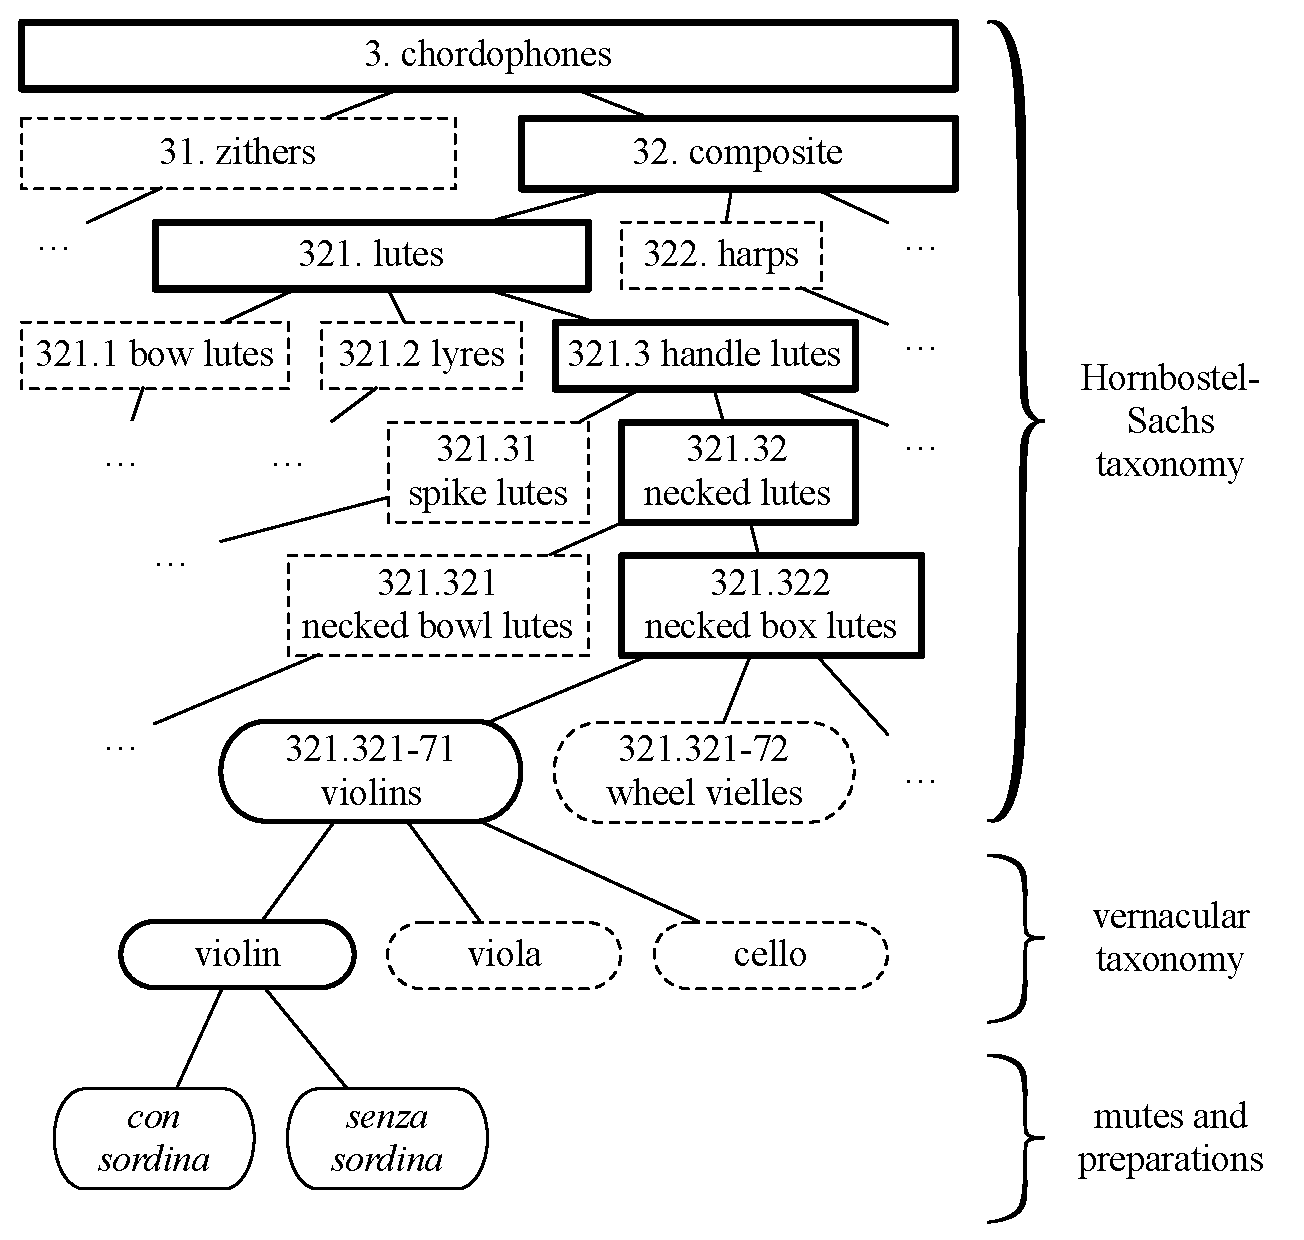
\includegraphics[width=\linewidth]{./figs/dendrograms/instrument-dendrogram.eps}
\caption{Instrument taxonomy.}
\label{fig:instrument-dendrogram}
\end{figure}


% Disentangling factors in variability in the production of musical sounds.

% Adopt the Visipedia approach.

% Distinguish what the left hand does from what the right hand does?
% Left hand: vibrato,
% Right hand: tremolo

% Bows and mallets are part of the gesture
% The use of mutes is part of the instrument BUT any gesture while holding the mute (e.g.  trombone) creates a new IPT category that is distinct from ordinary style.

% Out of scope are:
% Variations in articulation: trill, slide. Unlike vibrato, they have a melodic function.
% Variations in: artificial harmonics, subharmonics [ref Mari Kimura],
% Variations in phrasing: arpeggio,
% analog FX:

\ml{also describe the evaluation methodology. Ranking for compositional use, query by example, etc}

%%%%%%%%%%%%%%%%%%%%%%%%%%%%%%%%%%  METHODS  %%%%%%%%%%%%%%%%%%%%%%%%%%%%%%%%%%%
\section{Methods}
In this section, we point out the theoretical limitations of mel-frequency cepstral coefficients (MFCC) in the representation of musical sounds comprising with extended instrumental playing techniques (IPT), and describe how both the scattering transform and supervised metric learning may overcome such limitations.

\subsection{Limitations of mel-frequency cepstral coefficients}

\ml{not sure we need to discuss this. We should include the mfccs as baseline but more focus on what is needed: a representation of the data that is able to reliably consider larger frame sizes than usually considered}

\subsection{Scattering transform} % Scattering transform
\cite{anden2012dafx}

\section{Metric learning} % Large-margin nearest neighbors

As shown in the experiments described in Section \ref{sec:exp}, it is helpful to consider a supervised projection of the scattering coefficients in order to select among the large dimensionality of the resulting feature space, which axes are relevant for the task at hand.

May approaches can be considered to achieve such a task \cite{}. One standard approach is the use of the linear discriminant analysis (LDA) that linearly projects ($x \rightarrow L x$) the input data into a features space of $C$-1 dimensions that maximizes the amount of between-class variance
relative to the amount of within-class variance. The linear transformation $L$ is chosen to maximize the ratio of between-class to within-class variance,
subject to the constraint that $L$ defines a projection matrix.


A more flexible approach often taken in metric learning \cite{bellet2013survey} is to optimize a malahanobis matrix that linearly projects the input data into another feature space of the same dimensionality. In this case:
\begin{equation}
  M=L^T L
\end{equation}
and the resulting distance cane be expressed as follows:
\begin{equation}
  D_m(x, y) = (x_i-x_j)^T M(x_i-x_j)
\end{equation}
$x_i$ $x_j$ being features vectors. In this study, the large-margin nearest neighbors (LMNN) approach \cite{weinberger2006distance, weinberger2009distance} that optimizes the above described performance metric is considered. During the learning process, the following constraints are enforced: : the
k nearest neighbors of any training instance should belong to the
same class of the training instance ( the "pull" constraint) while keeping away instances of other classes (the "push" constraint).




%%%%%%%%%%%%%%%%%%%%%%%%%%%%%%%%%%%%%%%%%%%%%%%%%%%%%%%%%%%%%%%%%%%%%%%%%%%%%%%%
%%%%%%%%%%%%%%%%%%%%%%%%%%%% EXPERIMENTAL RESULTS %%%%%%%%%%%%%%%%%%%%%%%%%%%%%%
\section{Experimental results} \label{sec:exp}
In this section, we apply the aforementioned methods to instrument playing techniques classification in the Studio On Line (SOL) dataset of musical instrument samples for spectralist orchestration.

\subsection{Studio On Line (SOL) dataset}

The Studio On Line (SOL) dataset have been recorded at Ircam and is part of the orchestration tools developed in the institute. It is composed of 25444 recordings of single tones played by 16 musical instruments: Accordion, Alto, Bass, Bassoon, Clarinet, Contrabass, Flute, Guitar, Harp, Horn, Oboe, Tenor, Trumpet, Viola, Violin, and Violoncello. The number of recordings per class of instrument is on average 1590 $\pm$936.  Each instrument is played at different nuance and pitch if relevant using 143 different playing technique. The average number of number playing techniques is 178 $\pm$429. The large variance is due to the fact that some playing techniques may be considered for many instruments such as \textit{ordinario}, whereas other are specific to some instruments such as \textit{flatterzunge}. Figure \ref{fig:pt} shows the playing techniques with the higher, lower and median number of recordings.

%\begin{figure}
%\includegraphics[width=\textwidth,height=0.8\textheight,keepaspectratio]{./figs/solStats}
%\label{fig:pt}
%\end{figure}

\subsection{Musical instruments typology as reference}

In this section, we report experimental results while considering the musical instruments as the reference. Thus the task aims at grouping together in the feature space, recordings that are played by the same musical instrument regardless of the nuance, pitch and playing technique.

Baseline choice:
cut: keep lowest 13 over 40
std: remove mean divide by variance
\begin{tabular}{lllc}
features & cut & standardize & p (\%) \\
\hline
mfcc & 0 & 0 & 85 \\
mfcc & 0 & 1 & 84 \\
mfcc & 1 & 0 & 88 \\
mfcc & 1 & 1 & \textbf{\textcolor{red}{89}} \\
mel &  & 0 & 53 \\
mel &  & 1 & 50 \\
\end{tabular}

Scattering setting:
\begin{tabular}{lllc}
median & compress & standardize & p (\%) \\
\hline
0 & 0 & 0 & 64 \\
0 & 0 & 1 & 76 \\
0 & 1 & 0 & 84 \\
0 & 1 & 1 & 83 \\
1 & 0 & 0 & 77 \\
1 & 0 & 1 & 76 \\
1 & 1 & 0 & \textbf{\textcolor{red}{89}} \\
1 & 1 & 1 & 89 \\
\end{tabular}


\subsection{Instrumental playing technique typology as reference}

Baseline choice:
\begin{tabular}{lllc}
features & cut & standardize & p (\%) \\
\hline
mfcc & 0 & 0 & 35 \\
mfcc & 0 & 1 & 32 \\
mfcc & 1 & 0 & \textbf{\textcolor{red}{46}} \\
mfcc & 1 & 1 & 45 \\
mel &  & 0 & 19 \\
mel &  & 1 & 19 \\
\end{tabular}


\subsection{Discussion}


%%%%%%%%%%%%%%%%%%%%%%%%%%%%%%%%%%%%%%%%%%%%%%%%%%%%%%%%%%%%%%%%%%%%%%%%%%%%%%%%
%%%%%%%%%%%%%%%%%%%%%%%%%%%%%%%%%  CONCLUSION  %%%%%%%%%%%%%%%%%%%%%%%%%%%%%%%%%
\section{Conclusion}
Every quest for information is also a quest for invariance. [...]
% We have formulated the problem as query-by-example browsing. Another possible formulation would be textual description.

Our main finding is that mel-frequency cepstral coefficients (MFCC), although highly informative for musical instrument recognition in so-called ``ordinary'' notes, fail to discriminate extended instrumental techniques for at least three reasons.
First, they summarize spectral envelope without retaining its amplitude modulations.
Secondly, the frame rate at which they are computed ($T=\SI{25}{\milli\second}$ or so) is short enough to assume local stationarity, but not long enough to encompass all informative local correlations.
Thirdly, the discrete cosine transform (DCT) over mel frequencies does not, contrary to a widespread belief, make them invariant to the frequency transposition of complex sounds.
To address each of these shortcomings, we propose a simple pipeline of three elements: a time scattering transform; unsupervised metric learning over frequencies and modulation rates with large-margin nearest neighbors (LMNN); and a support vector machine (SVM) classifier.


\section{Acknowledgments}
% The authors wish to thank Andrew Farnsworth and (?) for fruitful discussions on Visipedia.
% Catherine Krocker for helpful suggestions on the title of this article.



% For bibtex users:
\bibliography{lostanlenPlayingTechniques}

\end{document}
